\chapter{Grundlagen}
\section{Funktionale Programmierung}
\section{Verwendete Programmiersprachen}
\subsection{Clojure}
\subsection{Elm}
\section{Eingesetzte Webtechnologien}
\subsection{Websockets}
\subsection{Single-Page-Applications}
\section{Microservices}
\section{Container-Virtualisierung mit Docker}
\begin{figure}
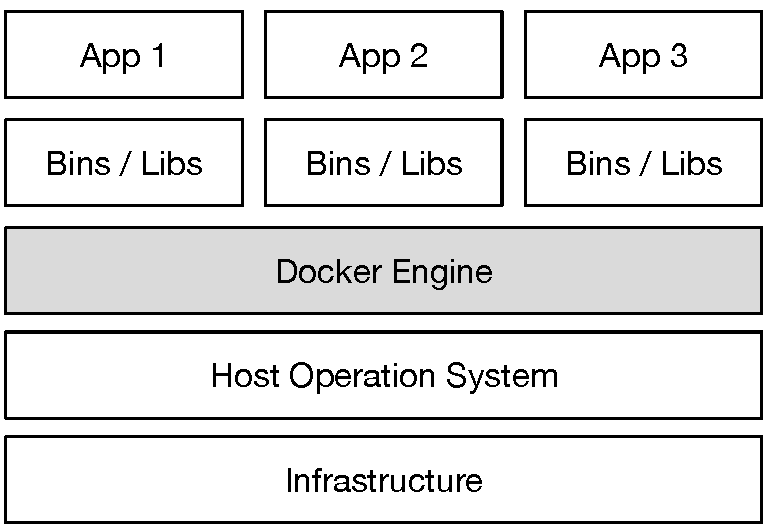
\includegraphics{docker.pdf}
\centering
\Large Schichten einer Visualisierung mit Docker
\par
[TODO: add figures to tof, figure-count]
\end{figure}
Docker\footnote{\link{https://docs.docker.com/}} ist eine Software zum Deployment von Applikationen innerhalb von Containern.
Im Vergleich zu \acp{VM}, ähnelt sich die Vorgehensweise, jedoch laufen die Prozesse der Container direkt auf dem Host-Betriebssystem.
Trotz dieser Tatsache sind die Prozesse mithilfe von \ac{u.A.} Control-Groups und Kernel Namespaces voneinander isoliert.
Weiterhin hat man die Möglichkeit mit gängigen Mandatory-Access-Control-Frameworks wie SE-Linux oder App-Armor die Rechte innerhalb der Container zu beschränken.
Als Anforderung besteht keine spezifische Hardware-Infrastruktur wie bei beispielsweise VMWare ESXi.
Ebenso ist Docker mittlerweile auf allen gängigen Betriebssystemen lauffähig, wobei Linux-Derivate die beste Unterstützung erhalten.
\par
Ein Container wird mithilfe eines Dockerfiles beschrieben.
Darin werden deskriptive Instruktionen definiert um Abhängigkeiten zu installieren, Konfigurationen vorzunehmen und andere Build-Steps auszuführen.
Ein spezifischer Container wird als Image bezeichnet und setzt sich aus granularen Sub-Images zusammen.
Beim Erzeugen von Images eigener Dockerfiles müssen im Vergleich zu \acp{VM} keine großen Dateien transferiert werden, da sie aus ihrem Rezept reproduzierbar sind. 
Es besteht auch die Möglichkeit, von anderen Dockerfiles zu erben und diese über das Netzwerk verteilt bereitzustellen.
Falls die über eine Docker-Registry angebotenen Schichten eines Containers noch nicht auf dem eigenen Rechner vorhanden sind, so werden diese heruntergeladen.
\par
Weiterhin gibt es einen entscheidenden Vorteil gegenüber einer traditionellen \ac{VM}: Ein Dockerfile trägt implizit zur Dokumentation bei, da jede Änderung an einem Container in seinem Rezept ergänzt werden muss, um diese bei einem erneuten Start \ac{bzw.} erneuten Build zu erhalten.
\par
Wird eine Applikation in einzelnen Services aufgeteilt, so bietet sich das Tool \textbf{Docker-Compose}\footnote{\link{https://docs.docker.com/compose/overview/}} an.
Es ermöglicht in einer einzelnen Datei (\texttt{docker-\break compose.yml}) alle Konfigurations-Parameter der einzelnen Containern zu definieren.
Das können \ac{bspw.} Volume-Mounts, Ports, Environment-Variables oder Netzwerke sein, welche sonst bei jedem \texttt{docker exec} Command angegeben werden müssten.
Alternativ dazu stünden eigene und oft fehlerintensive Shell-Scripts um ähnliches zu erreichen. 
\par
Es bietet sich auch an, getrennte Environments für Development, Test und Production als zentrale Dokumentation der Applikation zu nutzen (\texttt{docker-\break compose.[env].yml}).

\section{Apache Kafka}
Zwei\footnote{\link{https://kafka.apache.org/documentation/}}

